\chapter{Input und Output mit Files und Terminal}
\label{p:8}
%
%
Die zur Ein-/Ausgabe verwendeten Objekte \verb|cin| und \verb|cout|
sind (in \textit{iostream}) vordefinierte Variablen vom Klassentyp
\verb|stream|. Um von Files zu lesen bzw.\   auf Files zu schreiben
werden nun neue Streamvariablen angelegt und zwar vom
Typ \verb|ifstream| f"ur die Eingabe und vom Typ \verb|ofstream|
f"ur die Ausgabe. Der Filename wird beim Anlegen der Variablen "ubergeben
(C++ Konstruktor).
\index{Ausgabe!File}\index{Eingabe!File}
\index{Ausgabe!cout}\index{Eingabe!cin}
%\enlargethispage{28ex}
%
%
%\pagebreak[4]
\section{Kopieren von Files}
\label{p:8.1}
%
%
Das folgende Programm kopiert ein Inputfile auf ein Outputfile,
allerdings ohne Leerzeichen, Tabulatoren, Zeilenumbr"uche.
\includecode[firstline=3]{bsp811.cpp}{Files ohne Leerzeichen usw. kopieren}
Zeilenweises einlesen erfolgt über die Methode \texttt{getline()}.
%

Will man dagegen das File identisch kopieren, so mu"s auch
zeichenweise ein- und ausgelesen werden.
Hierzu werden die Methoden \verb|get| und \verb|put| aus
den entsprechenden Streamklassen verwendet.
\includecode[linerange={21-25}]{bsp812.cpp}{Identisches Kopieren von Files}
%
%

\section{Dateneingabe und -ausgabe via File}
\label{p:8.2}
%
%
Die Dateneingabe und -ausgabe via ASCII-File und Terminal kann gemischt
benutzt werden.
%\includecode[linerange={21-25}]{FileIO_a.cpp}{Dateingabe über File und Terminal}
\includecode[firstline=5]{FileIO_a.cpp}{Dateingabe über ASCII-File und Terminal}
%
%
Mehr Details, insbesondere zum binären Daten-I/O sind im \ghref{http://www.cplusplus.com/doc/tutorial/files/}{cplusplus-Tutorial} zu finden.
%
\section{Umschalten der Ein-/Ausgabe}
\label{p:8.3}
%
%%
%Manchmal ist ein problemabh"angiges Umschalten zwischen File-IO und
%Terminal-IO w"unschenswert oder n"otig.
%Leider mu"s in diesem Falle mit Zeigern auf die Typen
%\verb|istream| und \verb|ostream| gearbeitet werden.
%%\exfile{FileIO\_b.cpp}
%%\begin{latexonly}
%%\\[3cm]
%%\special{psfile=GIF/p99.eps.gz
%%	 hscale=15 vscale=15
%%	 voffset=-40
%%	}
%%\end{latexonly}
%%\begin{htmlonly} \\ \htmladdimg{p99_4.jpg}  \end{htmlonly}
%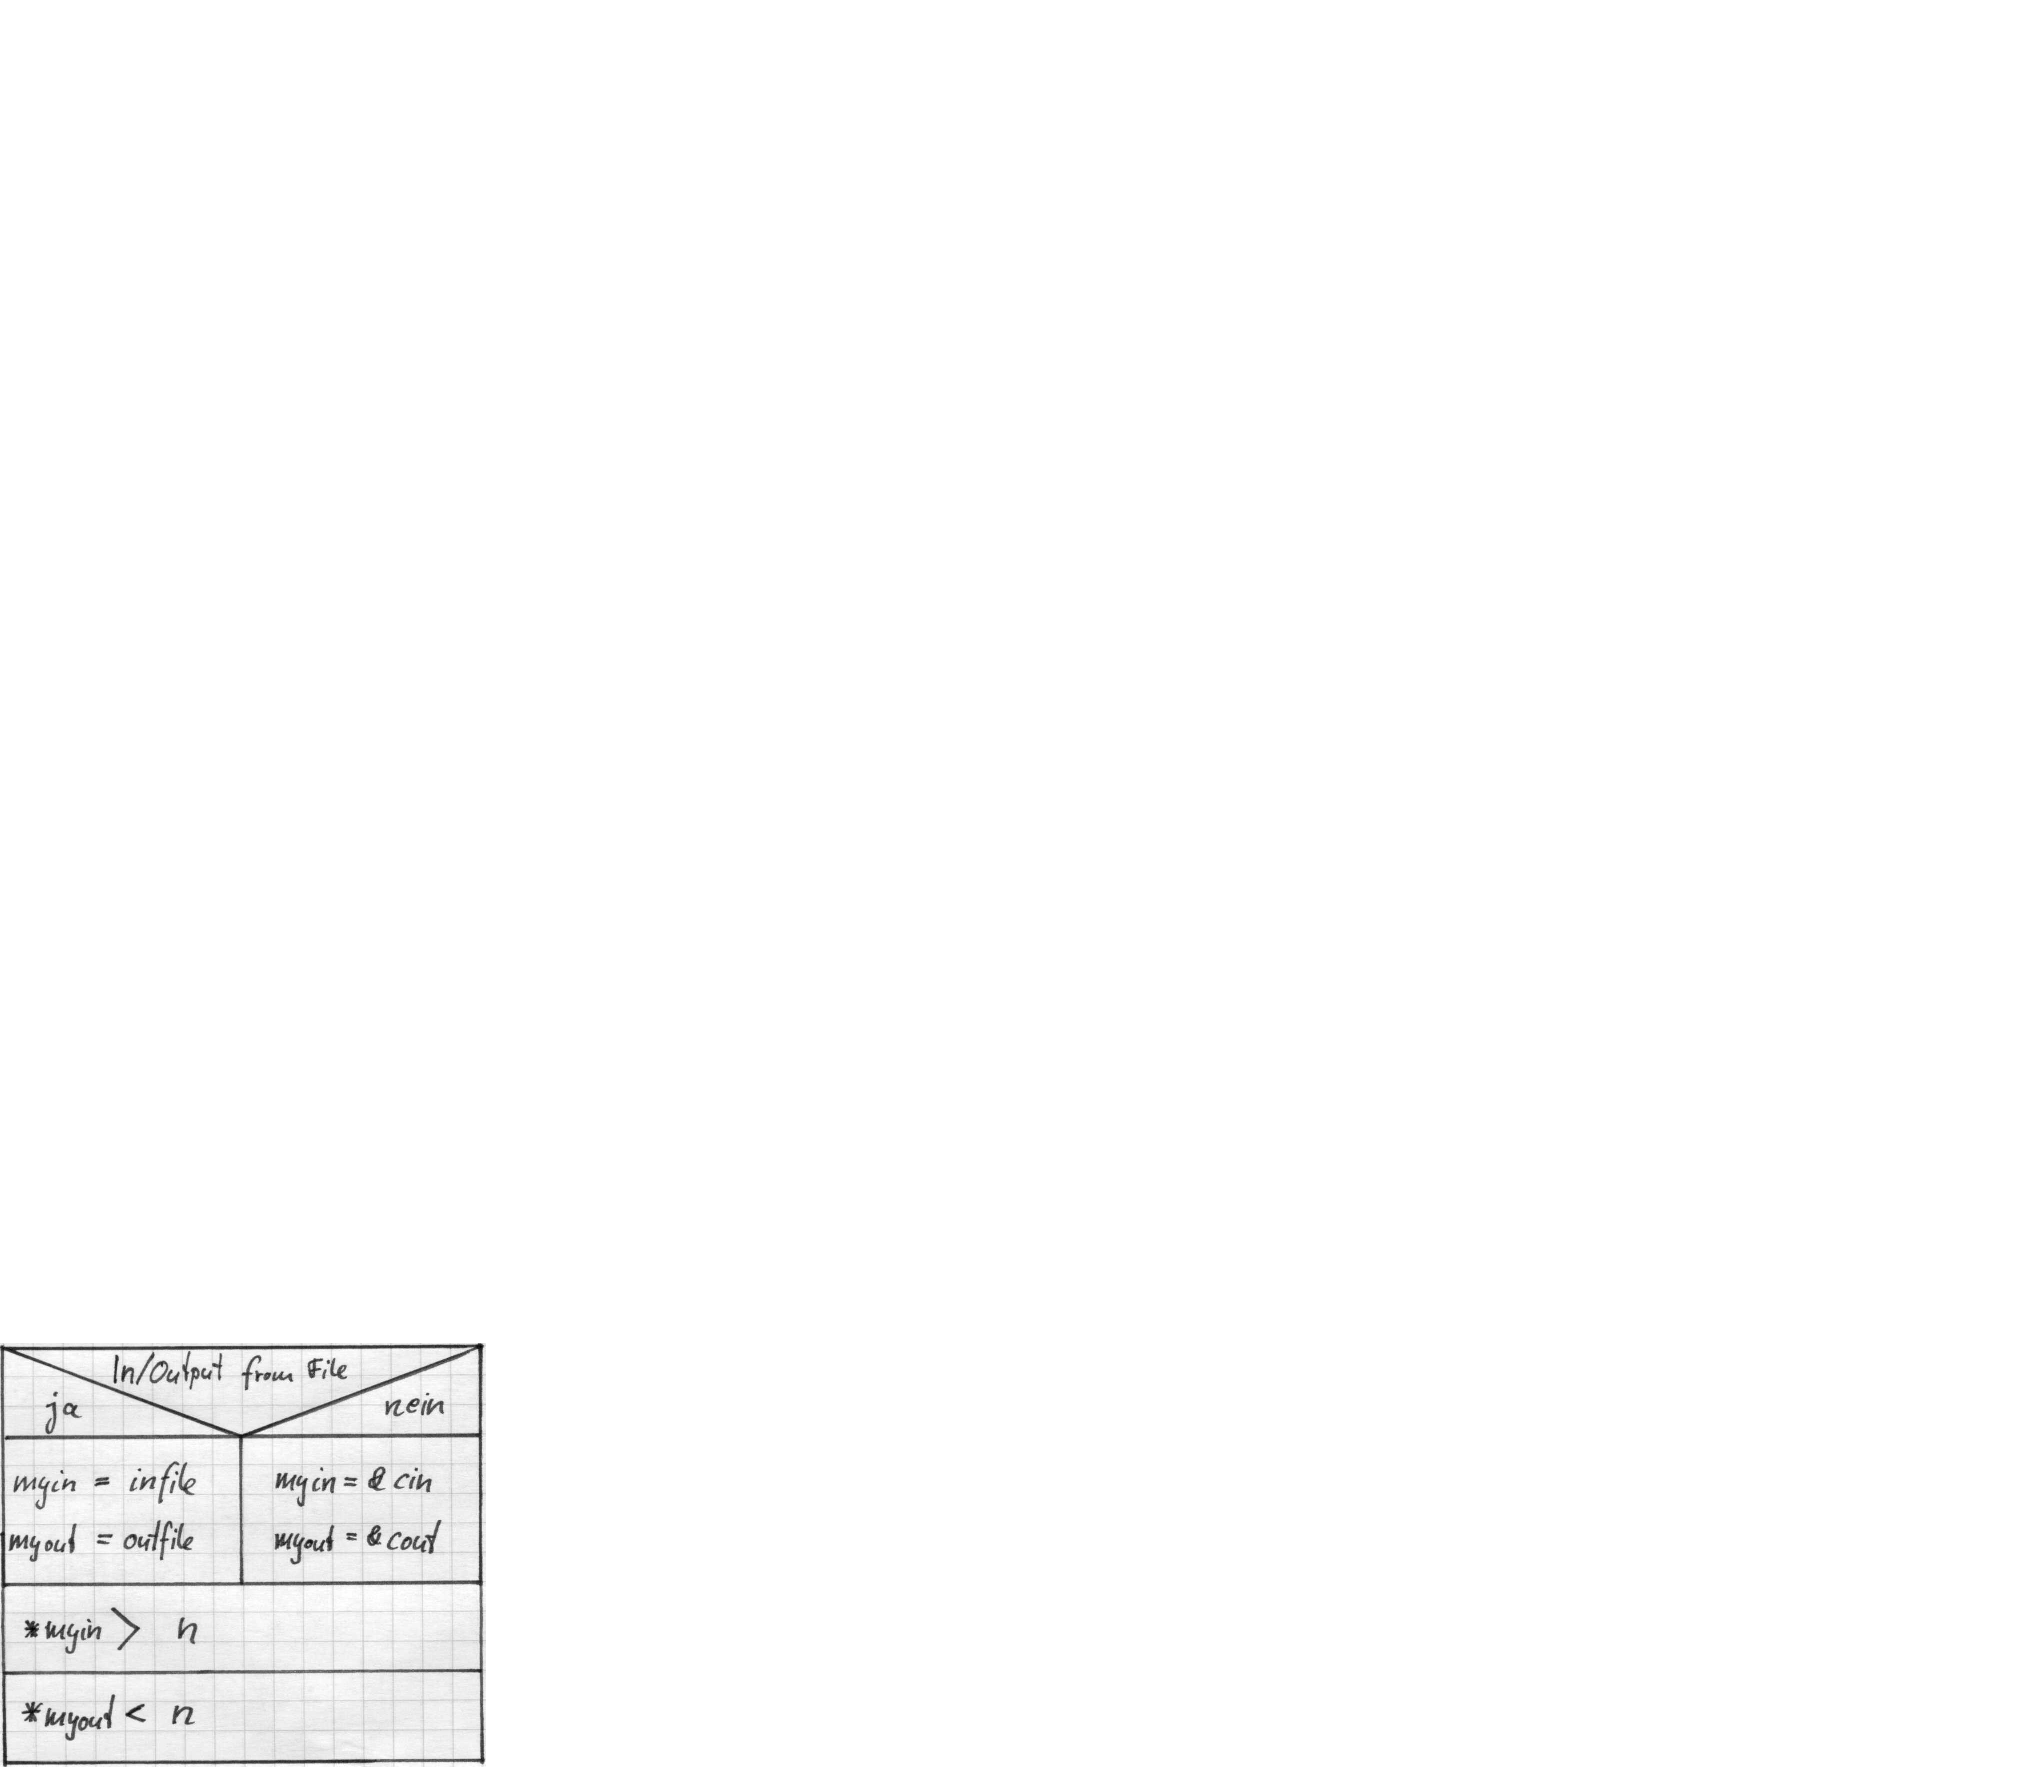
\includegraphics[scale=0.7]{GIF/p99}
%%
%\includecode[firstline=5]{FileIO_b.cpp}{Flexibles Umschalten zwischen File- und Terminal-IO}
%%
%In den Beispielen\bspfile{FileIO\_c.cpp}\bspfile{FileIO\_d.cpp} ist
%eine sehr komfortable M"oglichkeit des Umschaltens der Ein-/Ausgabe
%mittels Kommandozeilenparameter zu finden.

\begin{minipage}{0.5\textwidth}
Manchmal ist ein problemabh"angiges Umschalten zwischen File-IO und
Terminal-IO w"unschenswert oder n"otig.
Leider mu"s in diesem Falle mit Zeigern auf die Typen
\verb|istream| und \verb|ostream| gearbeitet werden.
\end{minipage} \hfill
\begin{minipage}{0.45\textwidth}
  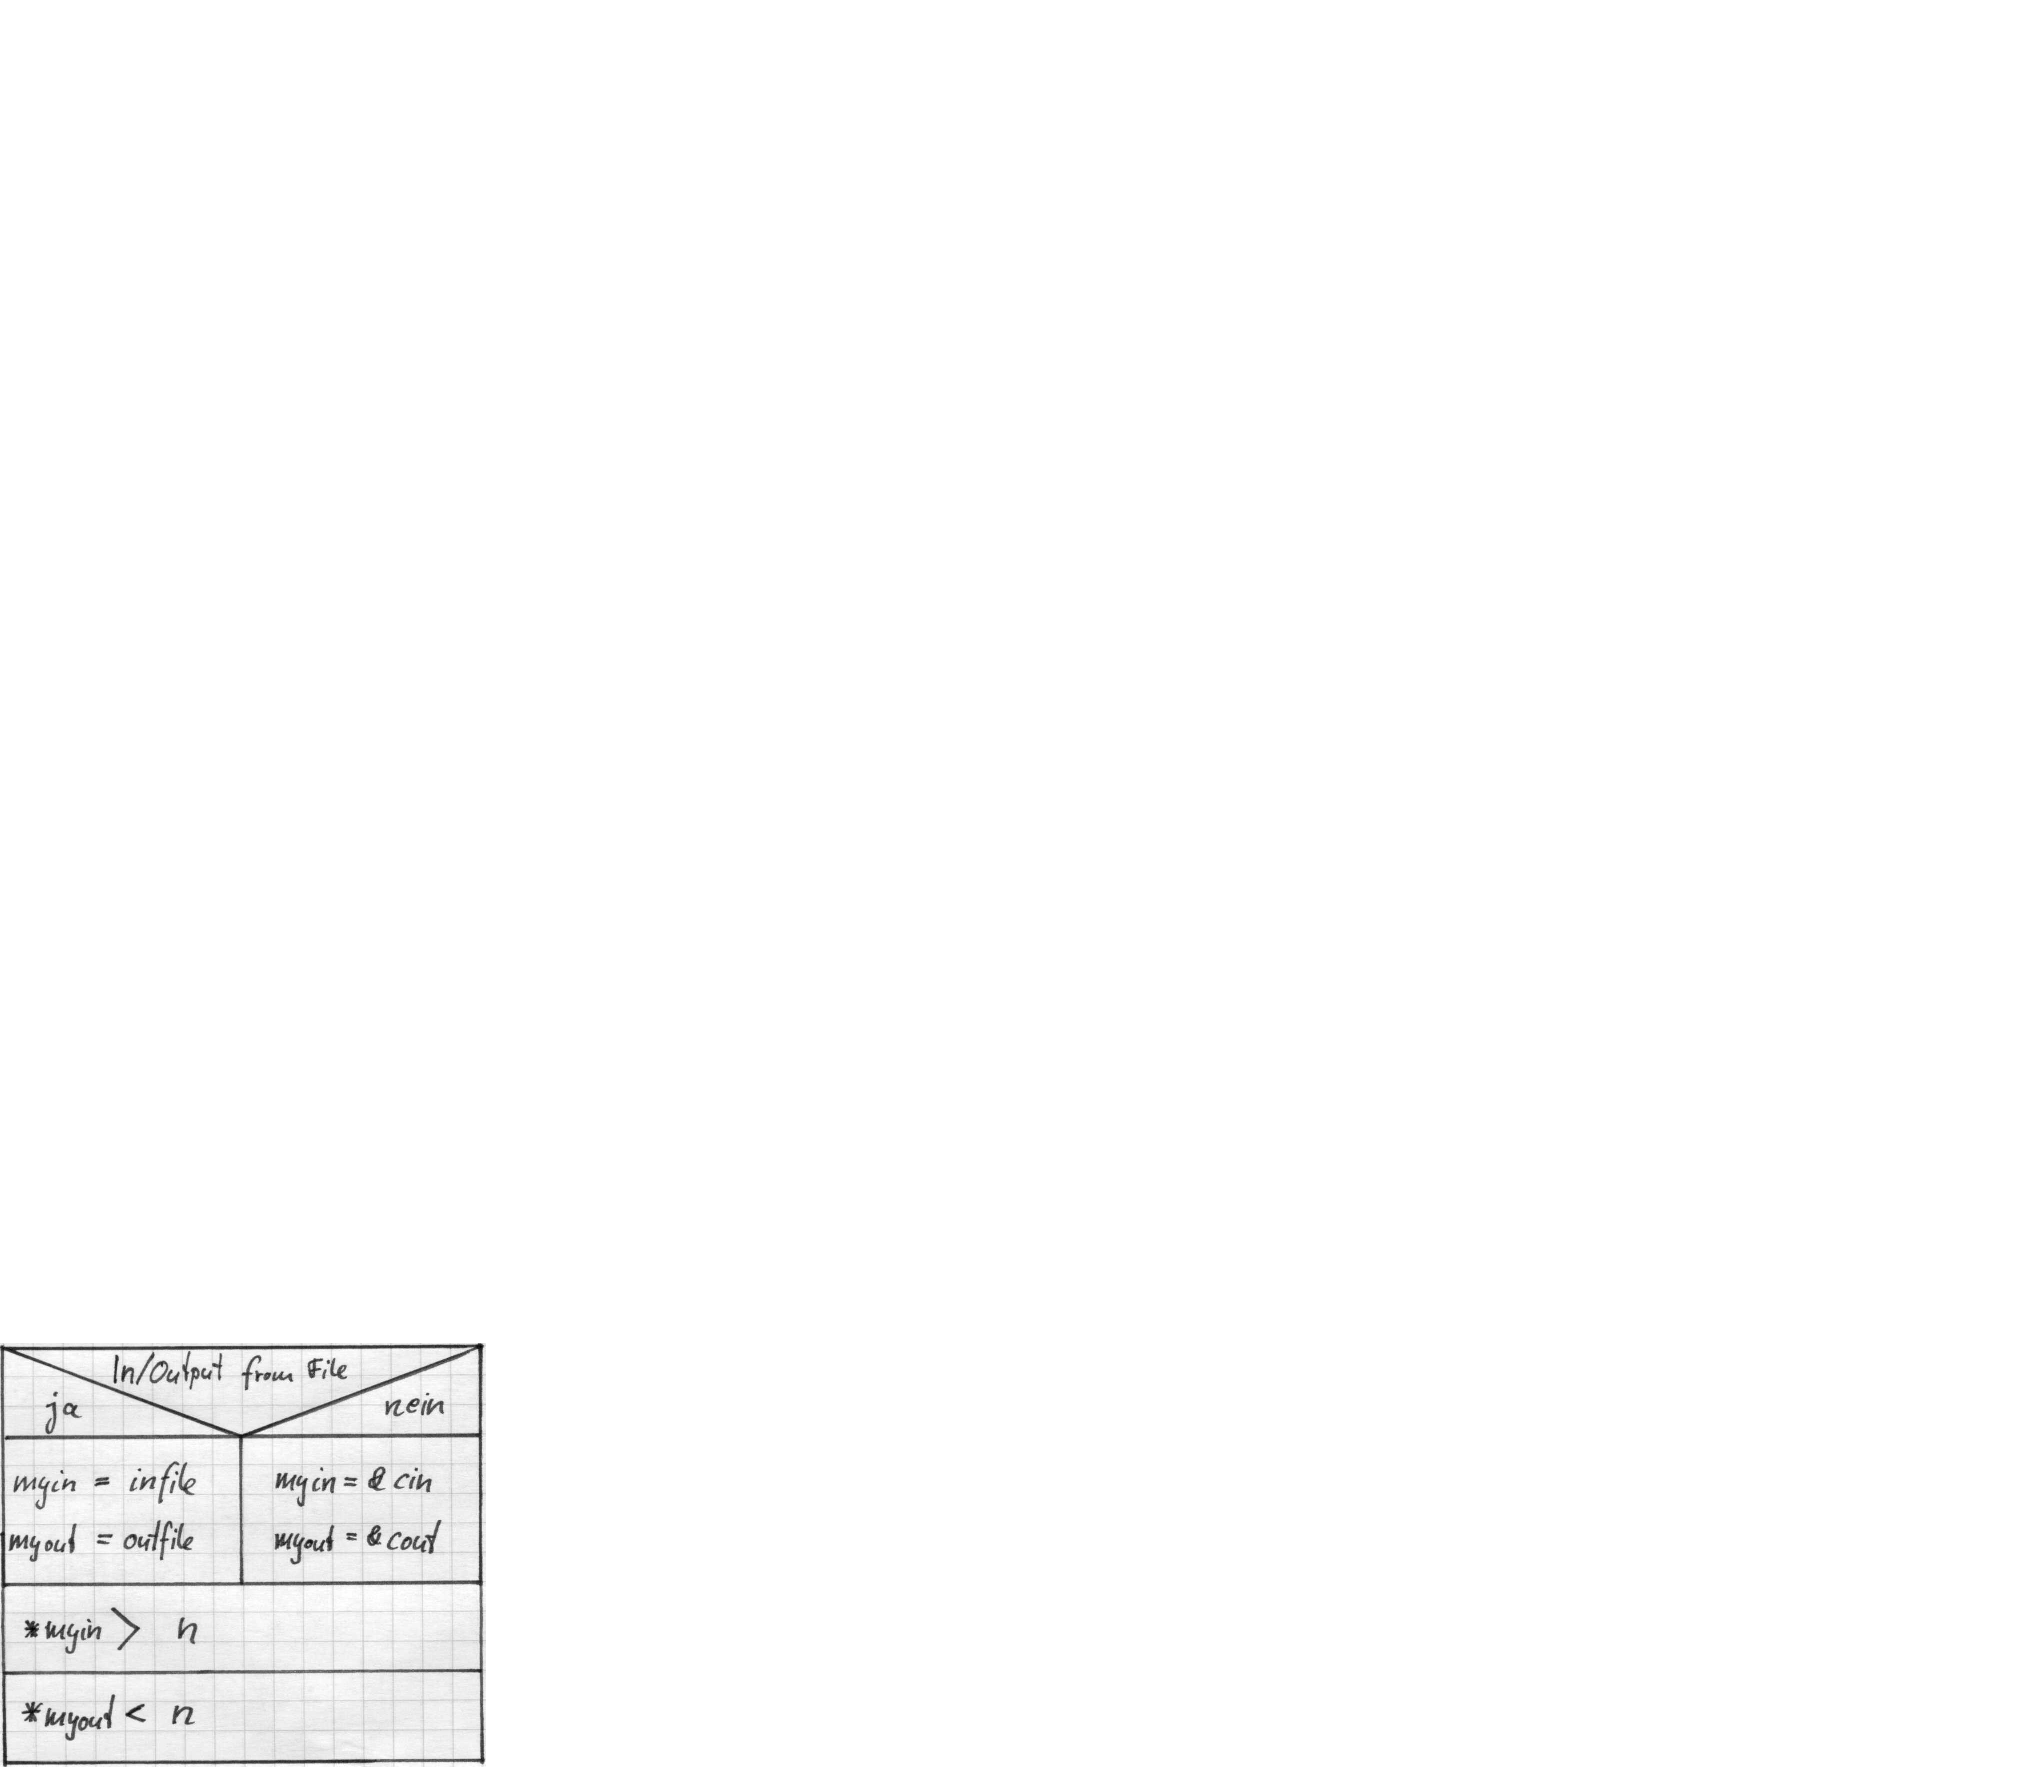
\includegraphics[scale=0.5]{GIF/p99}
\end{minipage}  
%\exfile{FileIO\_b.cpp}
%\begin{latexonly}
%\\[3cm]
%\special{psfile=GIF/p99.eps.gz
%	 hscale=15 vscale=15
%	 voffset=-40
%	}
%\end{latexonly}
%\begin{htmlonly} \\ \htmladdimg{p99_4.jpg}  \end{htmlonly}
\\
In den Beispielen\bspfile{FileIO\_c.cpp}\bspfile{FileIO\_d.cpp} ist
eine sehr komfortable M"oglichkeit des Umschaltens der Ein-/Ausgabe
mittels Kommandozeilenparameter zu finden.
%
\includecode[firstline=5]{FileIO_b.cpp}{Flexibles Umschalten zwischen File- und Terminal-IO}
%
%
\section{Ausgabeformatierung}
\label{p:8.4}
%
Die Ausgabe "uber Streams (\verb|<<|) kann verschiedenst formatiert
werden. Eine kleine Auswahl von Formatierungen sei hier angegeben,
mehr dazu in der Literatur \cite[\S7.2]{Wolf:2006:CAZ}
zu Manipulatoren und Methoden des
Input/Output--Streams.
\index{Ausgabe!Formatierung}
%

Wir benutzen die Variablen \bspfile{Format.cpp}
%
\hspace{2cm}
\begin{minipage}[t]{0.4\textwidth}
\begin{verbatim}
double da = 1.0/3.0,
       db = 21./2,
       dc = 1234.56789;
\end{verbatim}
\end{minipage}
%
\begin{itemize}
%
 \item Standardausgabe: \\
 	\verb|cout << da << endl << db << endl << dc << endl << endl;|
%
 \item Mehr g"ultige Ziffern (hier 12) in der Ausgabe:\\
 	\verb|cout.precision(12);| \\
	\verb|cout << ...|
%
 \item Fixe Anzahl (hier 6) von Nachkommastellen: \\
 	\verb|cout.precision(6);|  \\
 	\verb|cout.setf(ios::fixed, ios::floatfield);|  \\
	\verb|cout << ...|
%
 \item Ausgabe mit Exponent:\\
 	\verb|cout.setf(ios::scientific, ios::floatfield);|  \\
	\verb|cout << ...|
%
 \item R"ucksetzen auf Standardausgabe:\\
%  	\verb|cout.setf(0, ios::floatfield);|  \\
 	\verb|cout.setf(ios::floatfield);|  \\
	\verb|cout << ...|
%
 \item Ausrichtung (rechtsb"undig) und Platzhalter (16 Zeichen) via Methode \texttt{width}
       oder Manipulator \texttt{setw} welcher den Header
       \verb|<iomanip>| erfordert:\\
 	\verb|cout.setf(ios::right, ios::adjustfield);       //  Ausrichtung| \\
 	\verb|cout.width(16);                                //  Platzhalter|  \\
	\verb|cout << da << endl;| \\
 	\verb|cout.width(16);   cout << db << endl;| \\
      \verb|//  und nun Platzhalter via Manipulator| \\
	\verb|cout << setw(16) << da << setw(16) << db << endl << endl;| \\
	Die Nutzung von Standardmanipulatoren in der letzten Zeile ist
	in~\cite[\S1.4.6.2, pp.679]{Stroustrup:2000:CPP}
	zu finden.
%
 \item Hexadezimalausgabe von Integerzahlen: \\
% 	\verb|cout.setf(ios::hex, ios::basefield);| \\
%	\verb|cout << "127 = " << 127 << endl;| \\[0.5ex]
%	Alternativ via:\\
	\verb|cout << hex;|\\
	\verb|cout << "127 = " << 127 << endl;|
%
\item Ausgabe von Boolean:\\
	\verb|cout << boolalpha;|\\
	\verb|cout << true << " " << false << endl;|
%
\end{itemize}
%
%
%
\section{Abgesicherte Eingabe}
\label{p:8.5}
Tippfehler bei der Eingabe von Zahlen sind ärgerlich, insbesondere wenn dadurch das Programm in einer Endlosschleife der Eingabe hängenbleibt.
Dies läßt sich folgendermaßen absichern, die Idee dazu ist dem \ghref{http://www.cplusplus.com/articles/D9j2Nwbp/}{Beitrag in cplusplus.com} entnommen.
%
\includecode[firstline=6]{demoEingabe.cpp}{Für Integer abgesicherte Eingabe}
%
Obiges Beispiel kann allerdings keine Eingaben wie \verb| 3.5 |
statt der gewünschten \texttt{int}-Zahl~\verb| 3 | abfangen. 
Dafür wäre eine Konvertierung in \texttt{float} nötig.








